\documentclass[border=10pt]{standalone}
\usepackage{pgfplots}
\pgfplotsset{compat=1.18}
\begin{document}
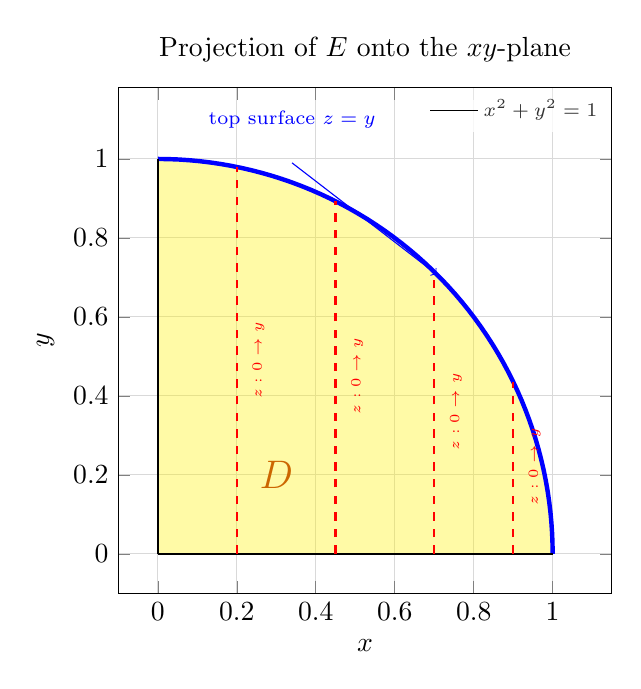
\begin{tikzpicture}
\begin{axis}[
    width=8cm, height=8cm, axis equal image,
    xmin=-0.1, xmax=1.15, ymin=-0.1, ymax=1.18,
    xlabel={$x$}, ylabel={$y$}, grid=major, grid style={black!15},
    title={Projection of $E$ onto the $xy$-plane},
    legend style={at={(1,1)},anchor=north east,draw=none,fill=white,fill opacity=.8,font=\scriptsize}]
  \addplot[fill=yellow, fill opacity=.35, draw=none, domain=0:90, samples=60] ({cos(x)},{sin(x)}) -- (0,0) -- cycle;
  \node[orange!80!black, font=\Large] at (axis cs:0.30,0.20) {$D$};
  \addplot[blue, ultra thick, domain=0:90, samples=60] ({cos(x)},{sin(x)});
  \addlegendentry{$x^2+y^2=1$}
  \addplot[black, thick] coordinates {(0,0) (1,0)};
  \addplot[black, thick] coordinates {(0,0) (0,1)};
  \addplot[red, dashed, thick] coordinates {(0.20,0) (0.20,0.9798)};
  \addplot[red, dashed, thick] coordinates {(0.45,0) (0.45,0.8930)};
  \addplot[red, dashed, thick] coordinates {(0.70,0) (0.70,0.7141)};
  \addplot[red, dashed, thick] coordinates {(0.90,0) (0.90,0.4359)};
  \node[red, font=\tiny, rotate=90] at (axis cs:0.255,0.49) {$z:0 \to y$};
  \node[red, font=\tiny, rotate=90] at (axis cs:0.505,0.45) {$z:0 \to y$};
  \node[red, font=\tiny, rotate=90] at (axis cs:0.755,0.36) {$z:0 \to y$};
  \node[red, font=\tiny, rotate=90] at (axis cs:0.955,0.22) {$z:0 \to y$};
  \draw[->, blue] (axis cs:0.34,0.99) -- (axis cs:0.7071,0.7071);
  \node[blue, font=\scriptsize] at (axis cs:0.34,1.10) {top surface $z=y$};
\end{axis}
\end{tikzpicture}
\end{document}
